\documentclass[final]{beamer}

\usepackage[scale=1.24]{beamerposter} % Use the beamerposter package for laying out the poster

\usetheme{confposter}

\setbeamercolor{block title}{fg=ngreen,bg=white} % Colors of the block titles
\setbeamercolor{block body}{fg=black,bg=white} % Colors of the body of blocks
\setbeamercolor{block alerted title}{fg=white,bg=dblue!70} % Colors of the highlighted block titles
\setbeamercolor{block alerted body}{fg=black,bg=dblue!10} % Colors of the body of highlighted blocks

%-----------------------------------------------------------
% Define the column widths and overall poster size
% To set effective sepwid, onecolwid and twocolwid values, first choose how many columns you want and how much separation you want between columns
% In this template, the separation width chosen is 0.024 of the paper width and a 4-column layout
% onecolwid should therefore be (1-(# of columns+1)*sepwid)/# of columns e.g. (1-(4+1)*0.024)/4 = 0.22
% Set twocolwid to be (2*onecolwid)+sepwid = 0.464
% Set threecolwid to be (3*onecolwid)+2*sepwid = 0.708

\newlength{\sepwid}
\newlength{\onecolwid}
\newlength{\twocolwid}
\newlength{\threecolwid}
\setlength{\paperwidth}{48in} % A0 width: 46.8in
\setlength{\paperheight}{36in} % A0 height: 33.1in
\setlength{\sepwid}{0.024\paperwidth} % Separation width (white space) between columns
\setlength{\onecolwid}{0.22\paperwidth} % Width of one column
\setlength{\twocolwid}{0.464\paperwidth} % Width of two columns
\setlength{\threecolwid}{0.708\paperwidth} % Width of three columns
\setlength{\topmargin}{-0.5in} % Reduce the top margin size
%-----------------------------------------------------------

\usepackage{graphicx}  % Required for including images

\usepackage{booktabs} % Top and bottom rules for tables




%----------------------------------------------------------------------------------------
%	TITLE SECTION
%----------------------------------------------------------------------------------------

\title{Research Title} % Poster title

\author{J. Russo, JJ Dong} % Author(s)

\institute{Bucknell University, Department of Physics and Astronomy} % Institution(s)


\begin{document}

\addtobeamertemplate{block end}{}{\vspace*{2ex}} % White space under blocks
\addtobeamertemplate{block alerted end}{}{\vspace*{2ex}} % White space under highlighted (alert) blocks

\setlength{\belowcaptionskip}{2ex} % White space under figures
\setlength\belowdisplayshortskip{2ex} % White space under equations

\begin{frame}[t] % The whole poster is enclosed in one beamer frame
\begin{columns}[t] % The whole poster consists of three major columns, the second of which is split into two columns twice - the [t] option aligns each column's content to the top

\begin{column}{\sepwid}\end{column} % Empty spacer column


% ------------------------- First column -------------------------
\begin{column}{\onecolwid}

  %----------------------------------------------------------------------------------------
  %	Motivation
  %----------------------------------------------------------------------------------------

  \begin{alertblock}{Motivation/Background}

  \begin{itemize}
    \item Ubiquitous threat of antibiotic resistance
    \item Investigate effect of different cellular transformation rates on antibiotic
    resistant bacterial population growth
    \item Plasmids
  \end{itemize}

  \begin{center}
    Diagram of cell with plasmids
  \end{center}

  \end{alertblock}



  \begin{alertblock}{Constant $\alpha$}

  \begin{center}
    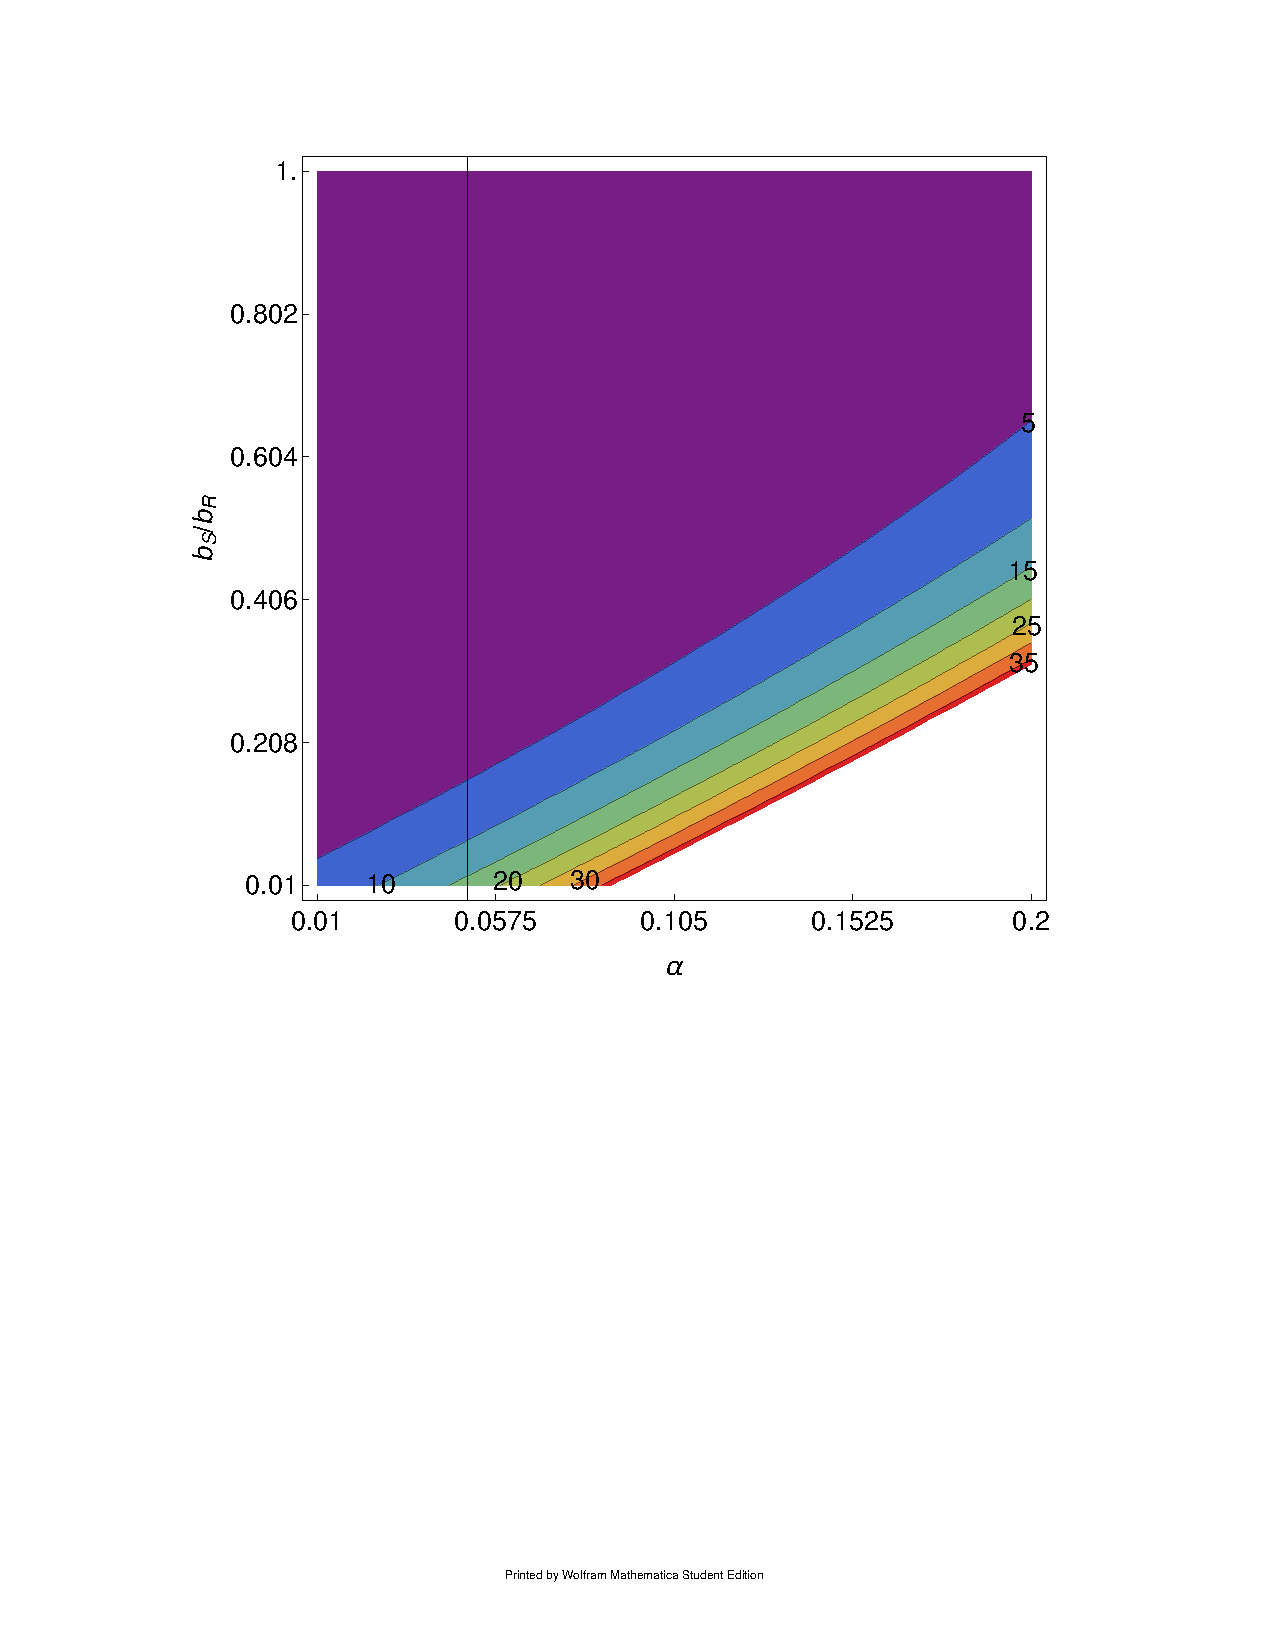
\includegraphics[width=0.9\columnwidth]{../dev/graphics/Jul14/const_alpha_contour.pdf}

    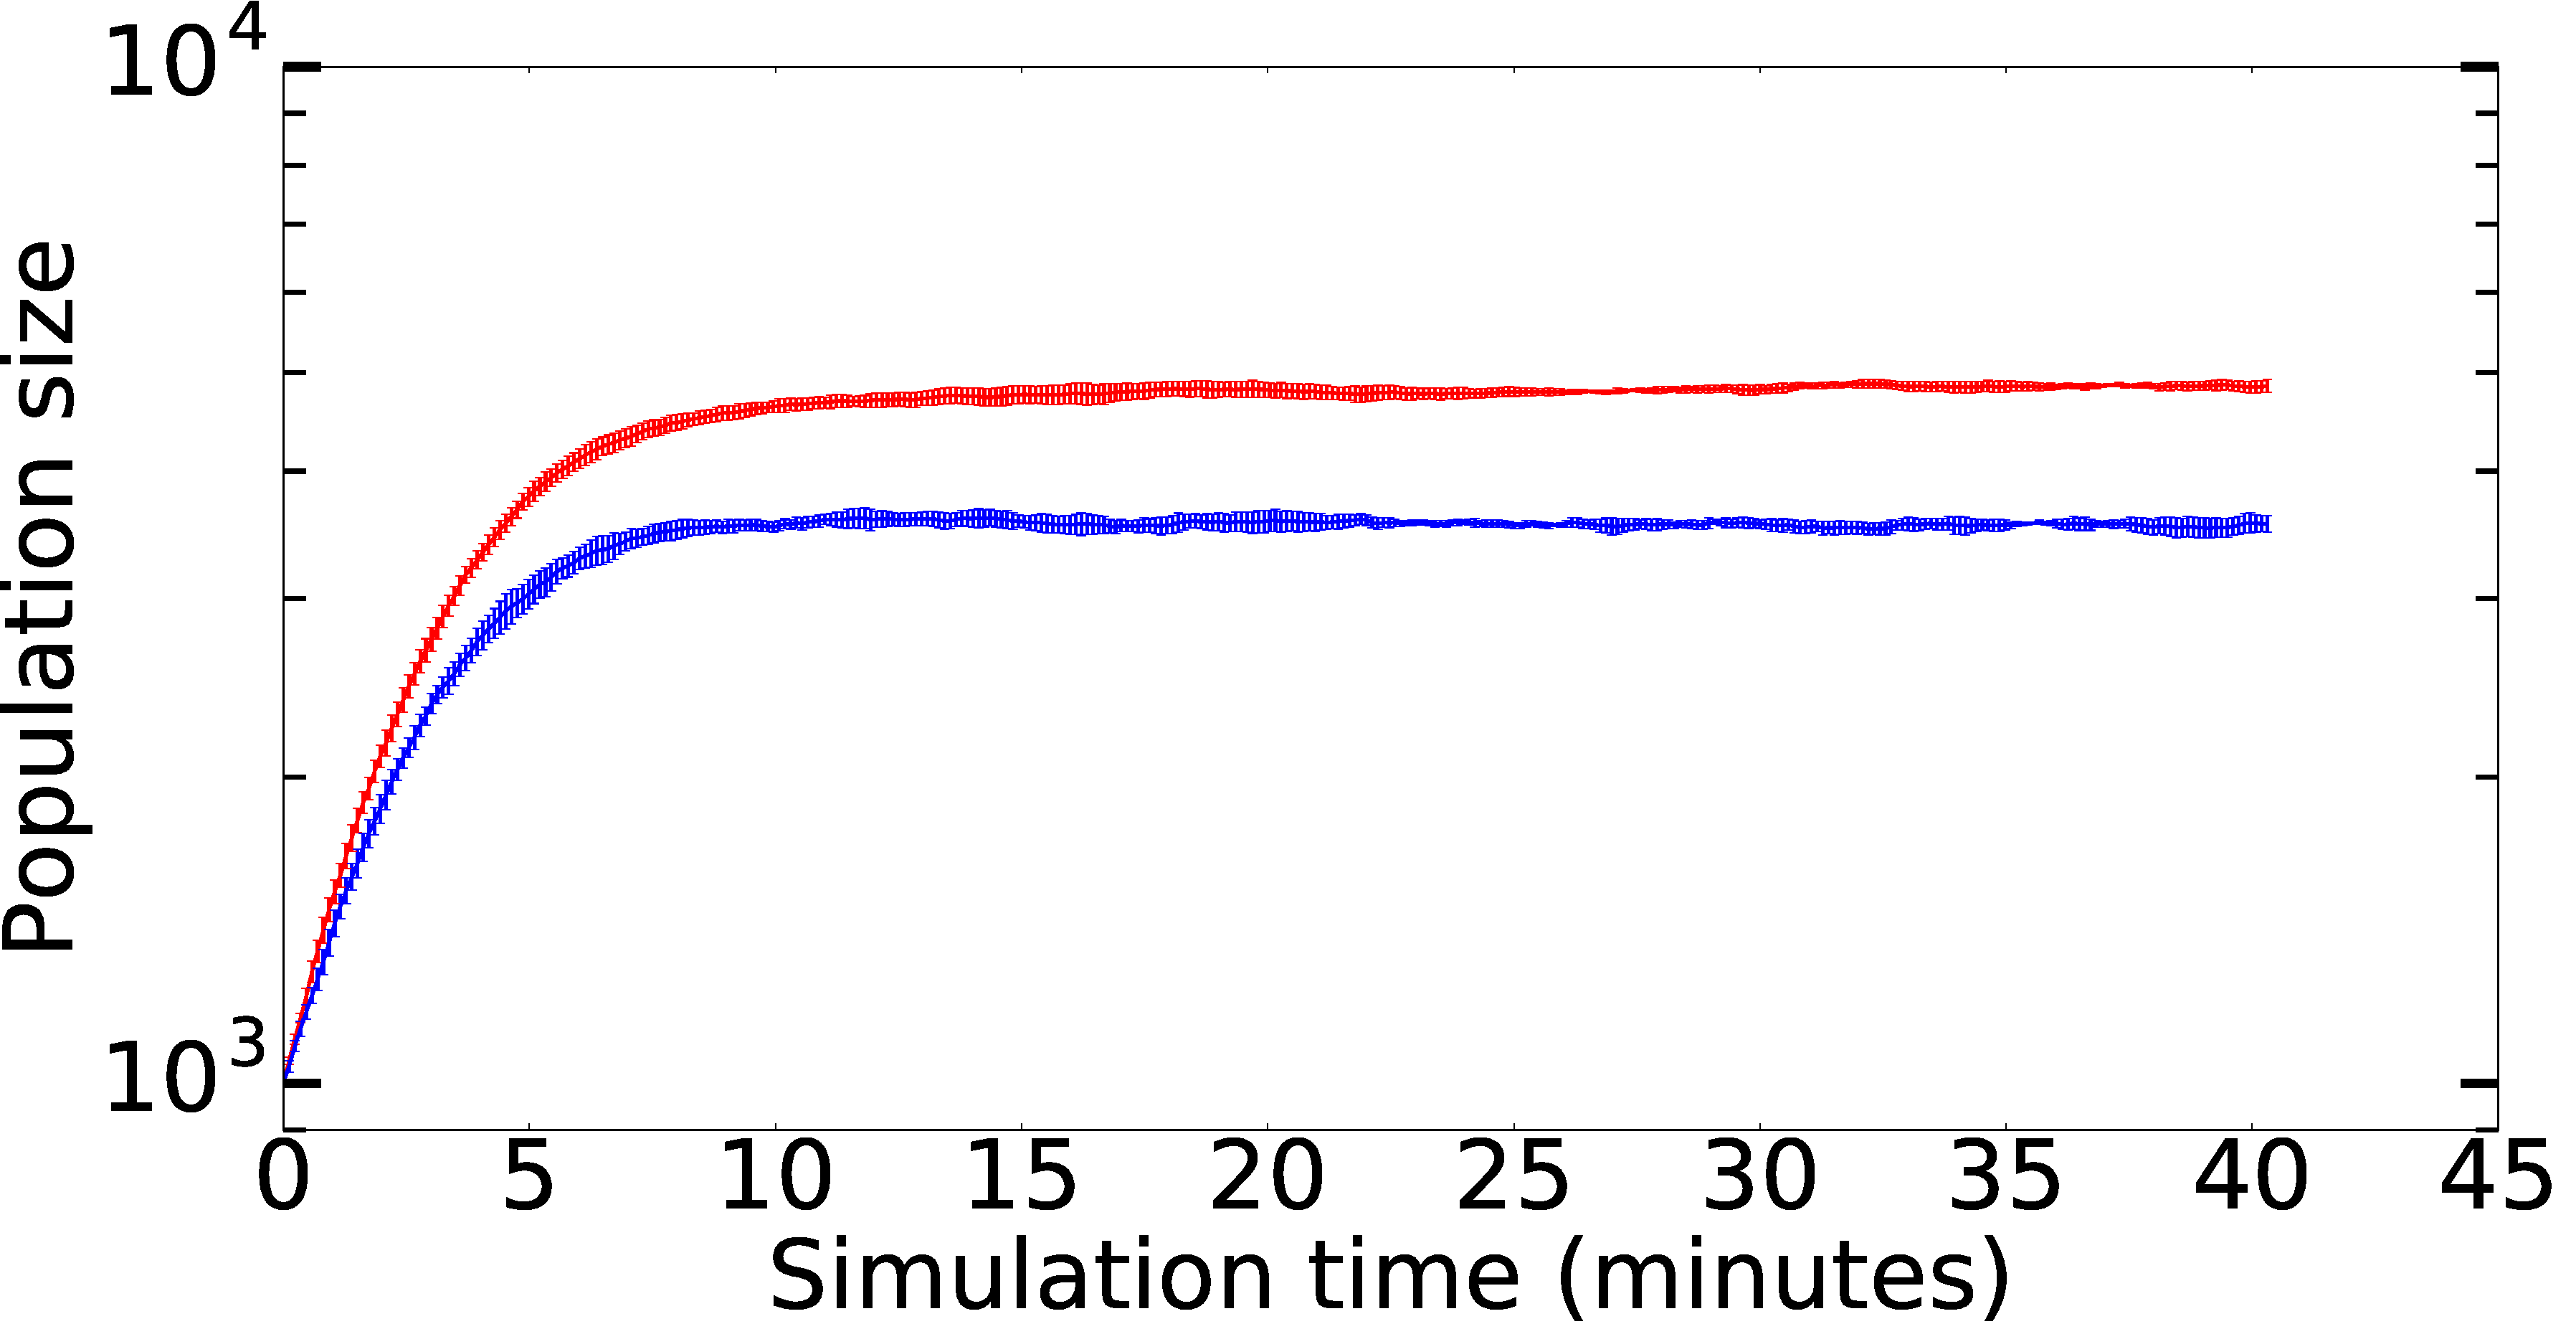
\includegraphics[width=0.9\columnwidth]{../dev/graphics/Jul18/const_pop.pdf}
  \end{center}

  \end{alertblock}

\end{column}
% ----------------------------------------------------------------
\begin{column}{\sepwid}\end{column} % Empty spacer column


% ------------------------- Second column -------------------------
\begin{column}{\onecolwid}



%----------------------------------------------------------------------------------------
%	INTRODUCTION
%----------------------------------------------------------------------------------------

\begin{block}{Simulation Methods}

\begin{itemize}
  \item Combined approach of Kinetic Monte Carlo simulation and numerical modeling
  \item Gillespie algorithm
  \item Well-mixed population
  \item Three cases
  \begin{itemize}
    \item Constant $\alpha$
    \item Linear $\alpha$
    \item Recycled $\alpha$
  \end{itemize}
\end{itemize}

\end{block}


    \begin{alertblock}{Linear $\alpha$}

    \begin{center}
      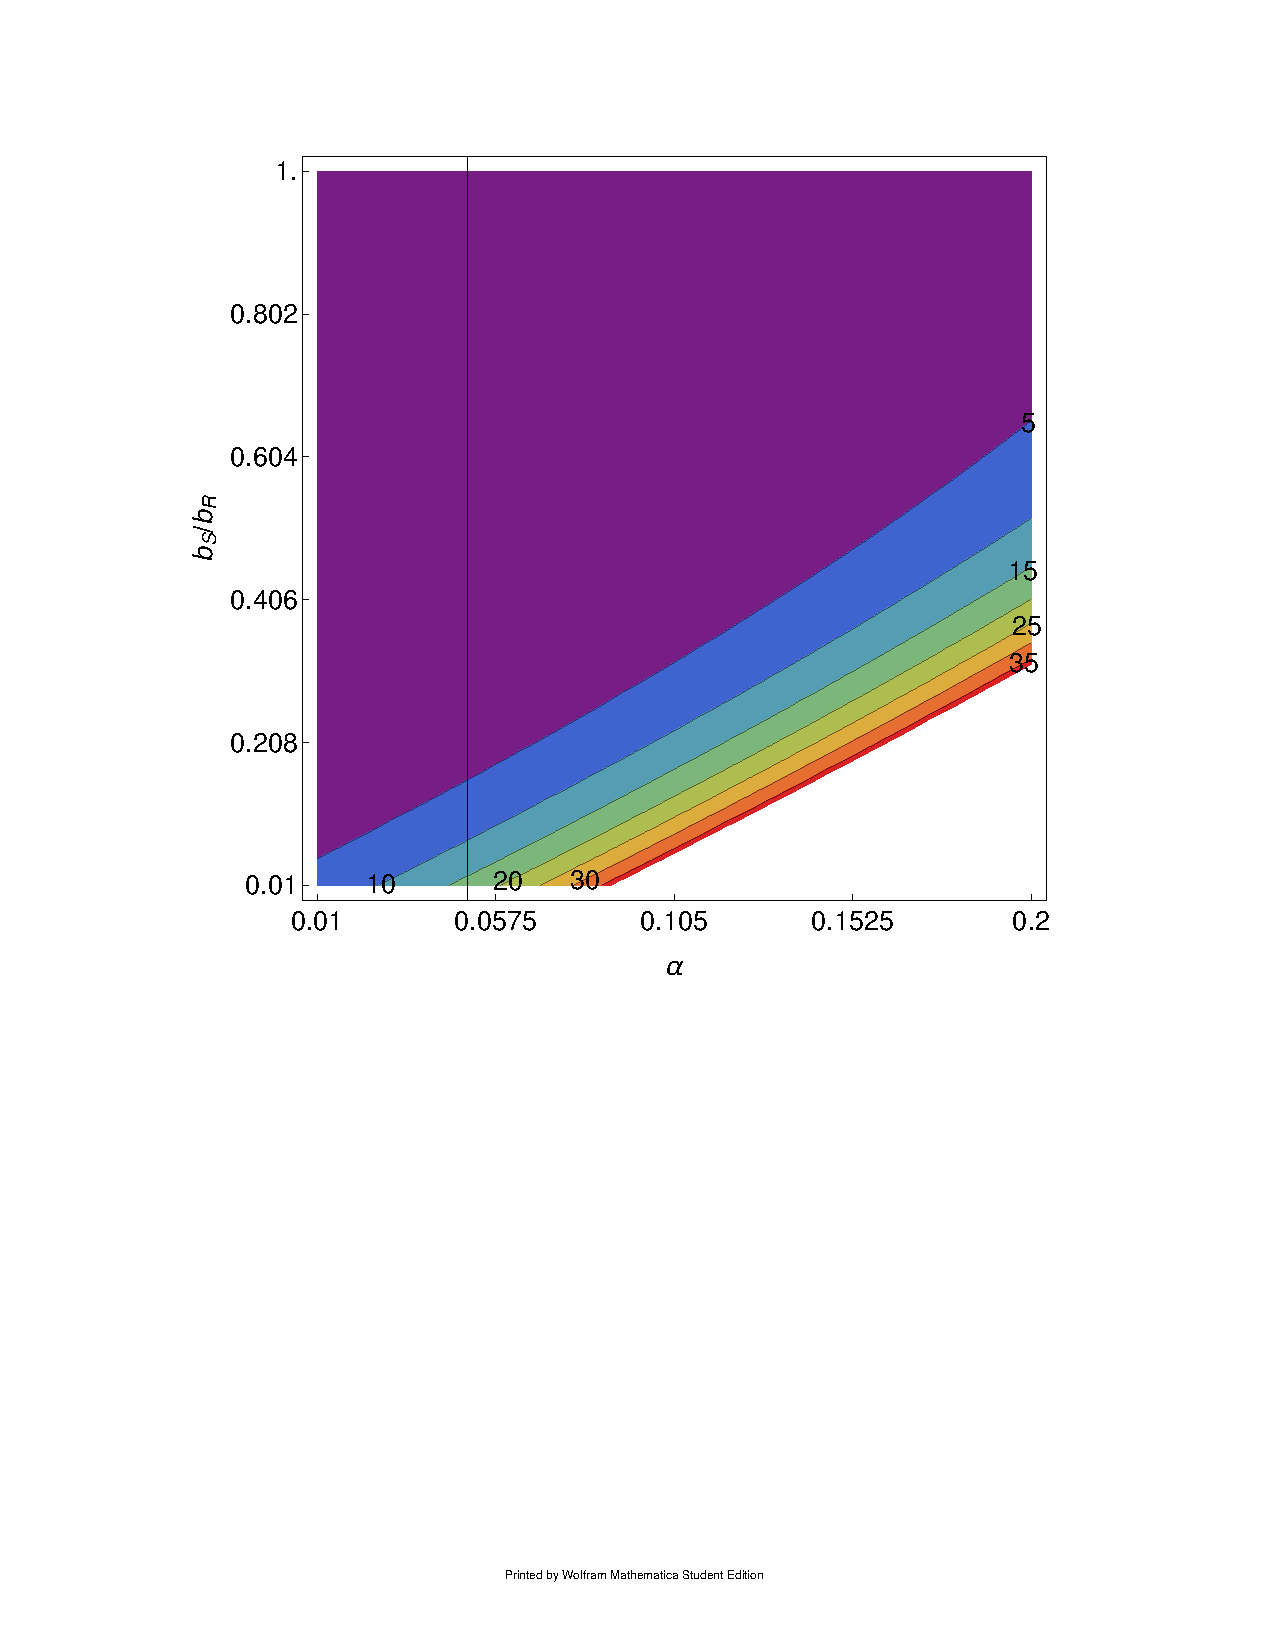
\includegraphics[width=0.9\columnwidth]{../dev/graphics/Jul14/const_alpha_contour.pdf}

      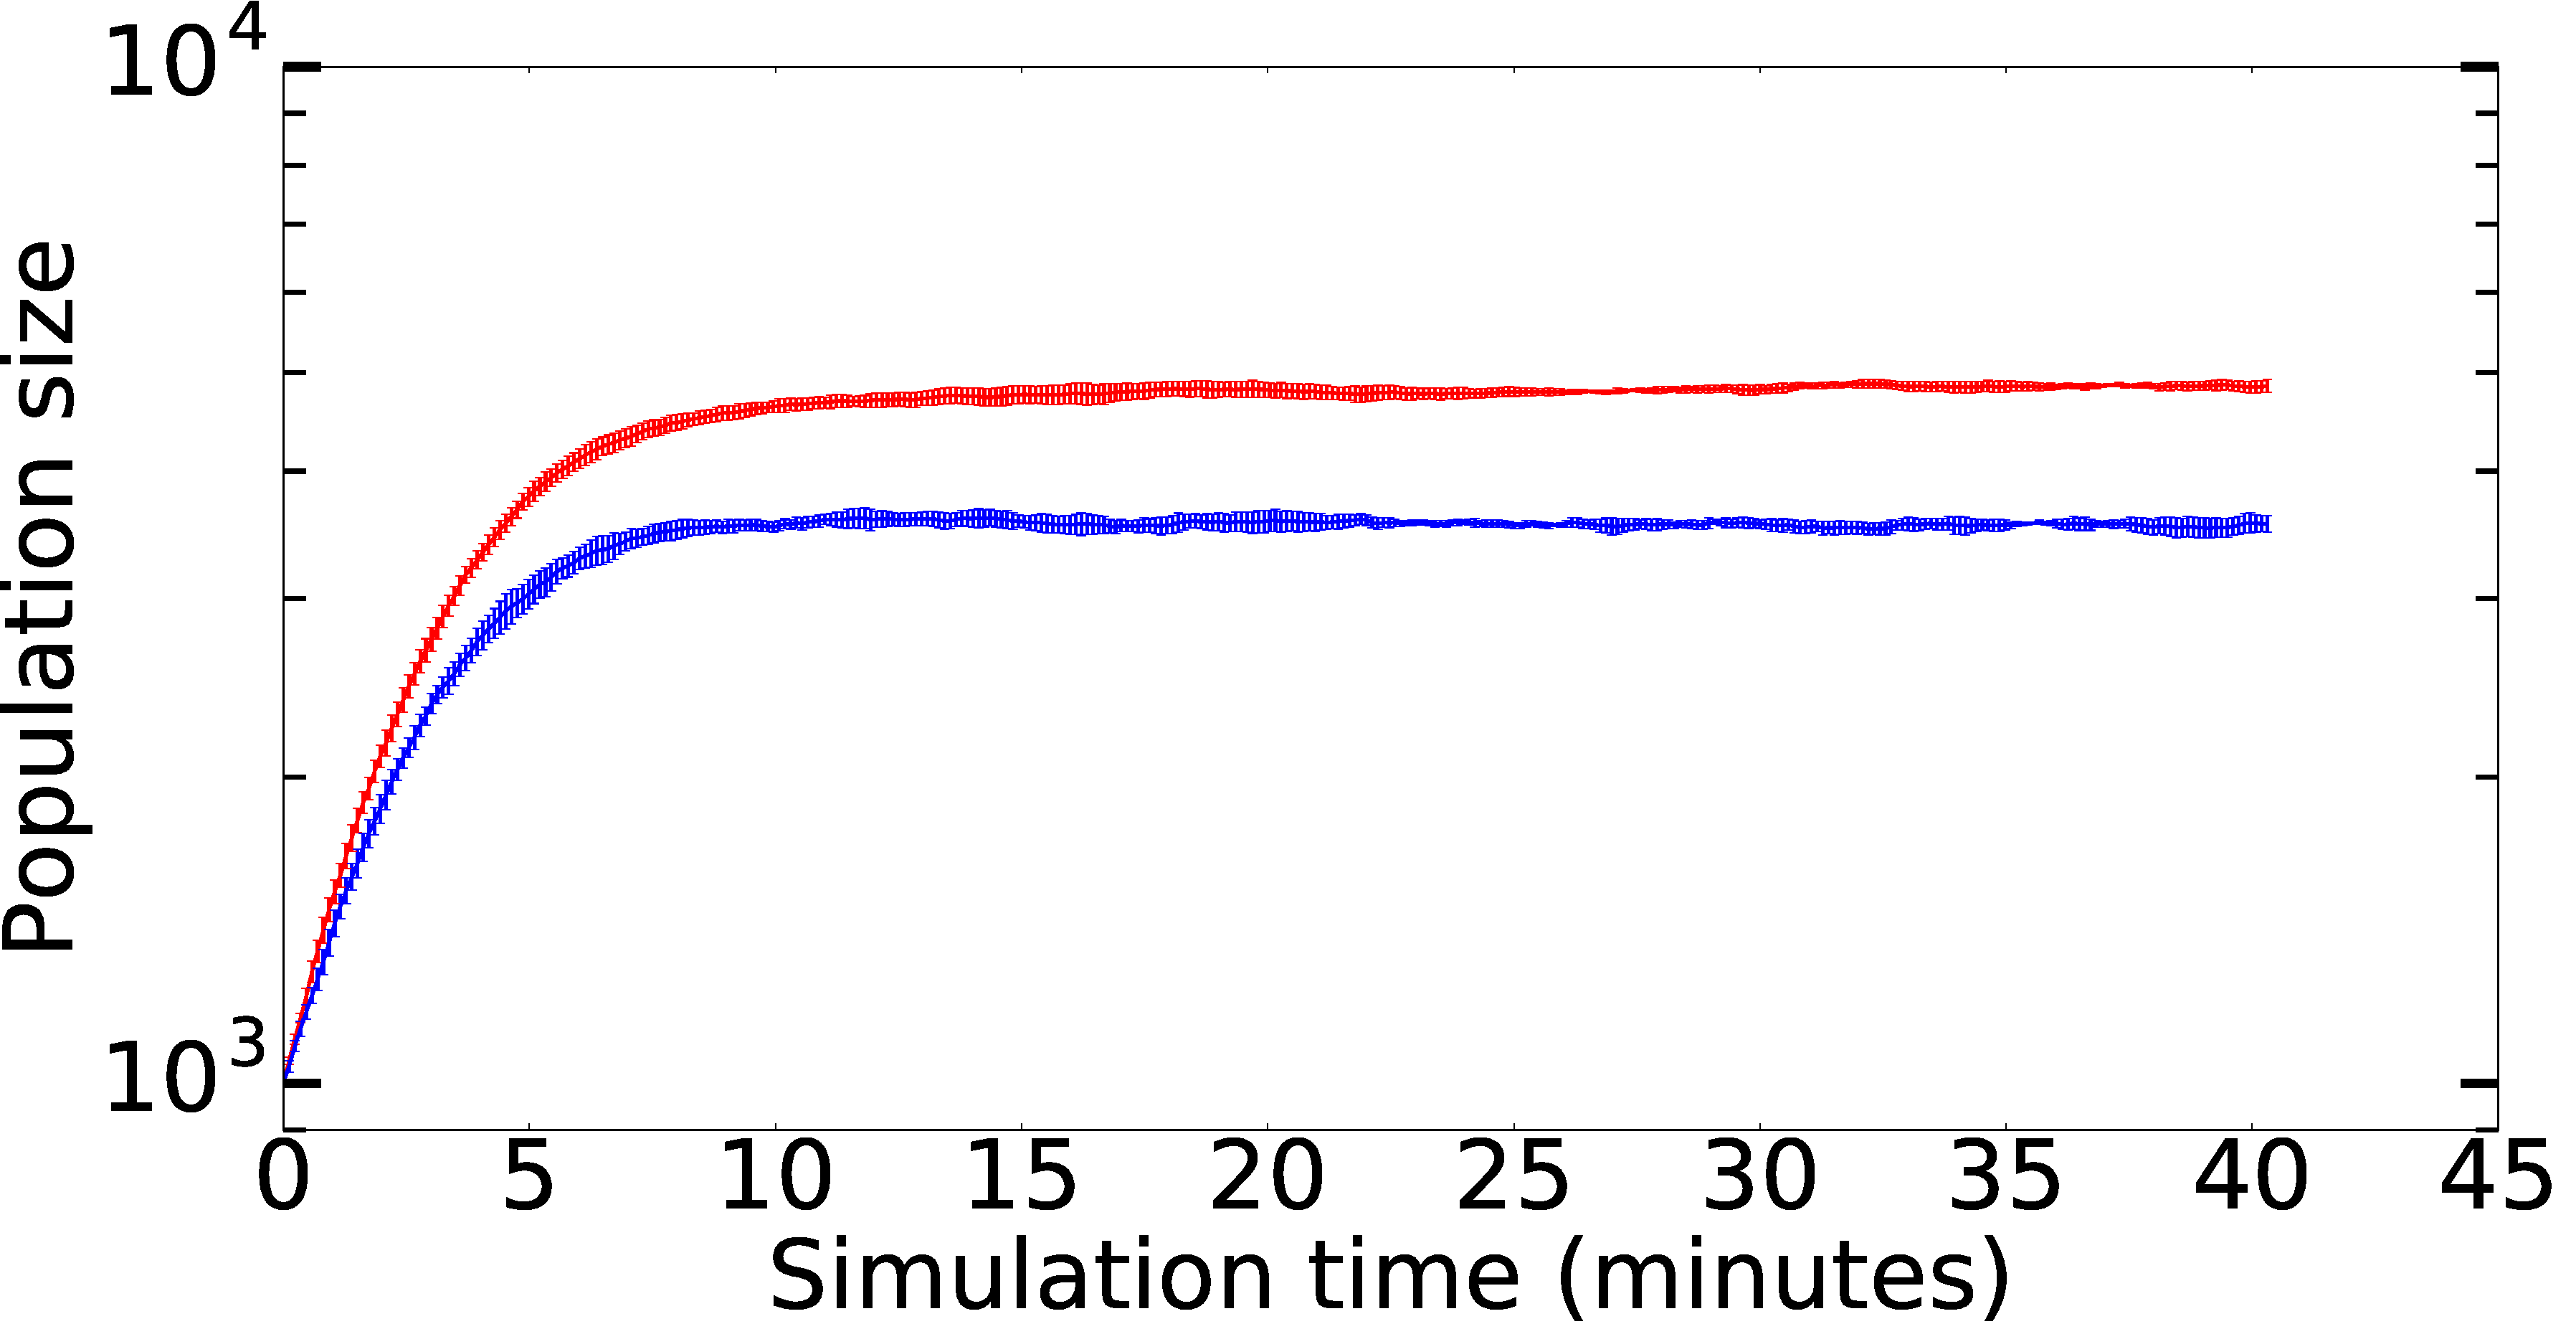
\includegraphics[width=0.9\columnwidth]{../dev/graphics/Jul18/const_pop.pdf}
    \end{center}

    \end{alertblock}
\end{column}
% ----------------------------------------------------------------
\begin{column}{\sepwid}\end{column} % Empty spacer column


% ------------------------- Third column -------------------------
\begin{column}{\onecolwid}




  %----------------------------------------------------------------------------------------
  %	INTRODUCTION
  %----------------------------------------------------------------------------------------

  \begin{block}{Simulation Methods}

  \begin{itemize}
    \item Combined approach of Kinetic Monte Carlo simulation and numerical modeling
    \item Gillespie algorithm
    \item Well-mixed population
    \item Three cases
    \begin{itemize}
      \item Constant $\alpha$
      \item Linear $\alpha$
      \item Recycled $\alpha$
    \end{itemize}
  \end{itemize}

  \end{block}



      \begin{alertblock}{Recycled $\alpha$}

      \begin{center}
        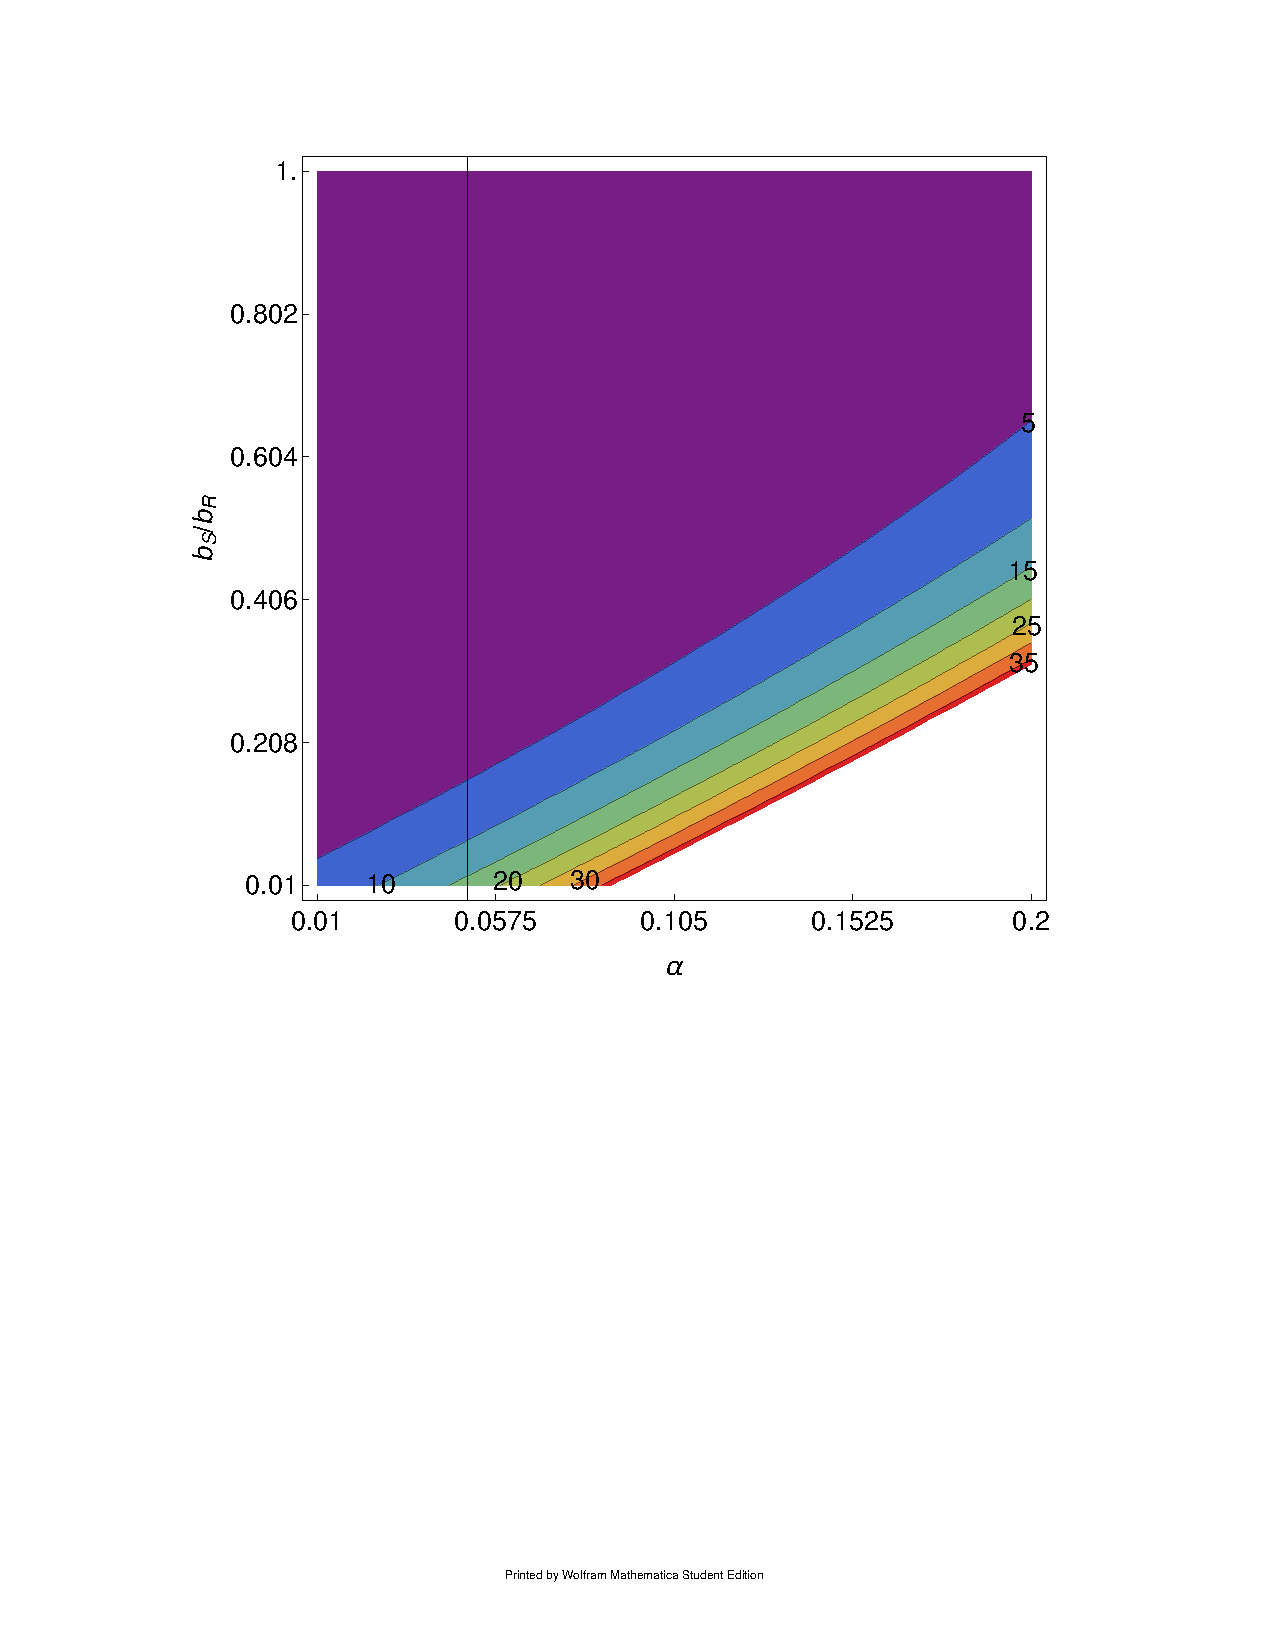
\includegraphics[width=0.9\columnwidth]{../dev/graphics/Jul14/const_alpha_contour.pdf}

        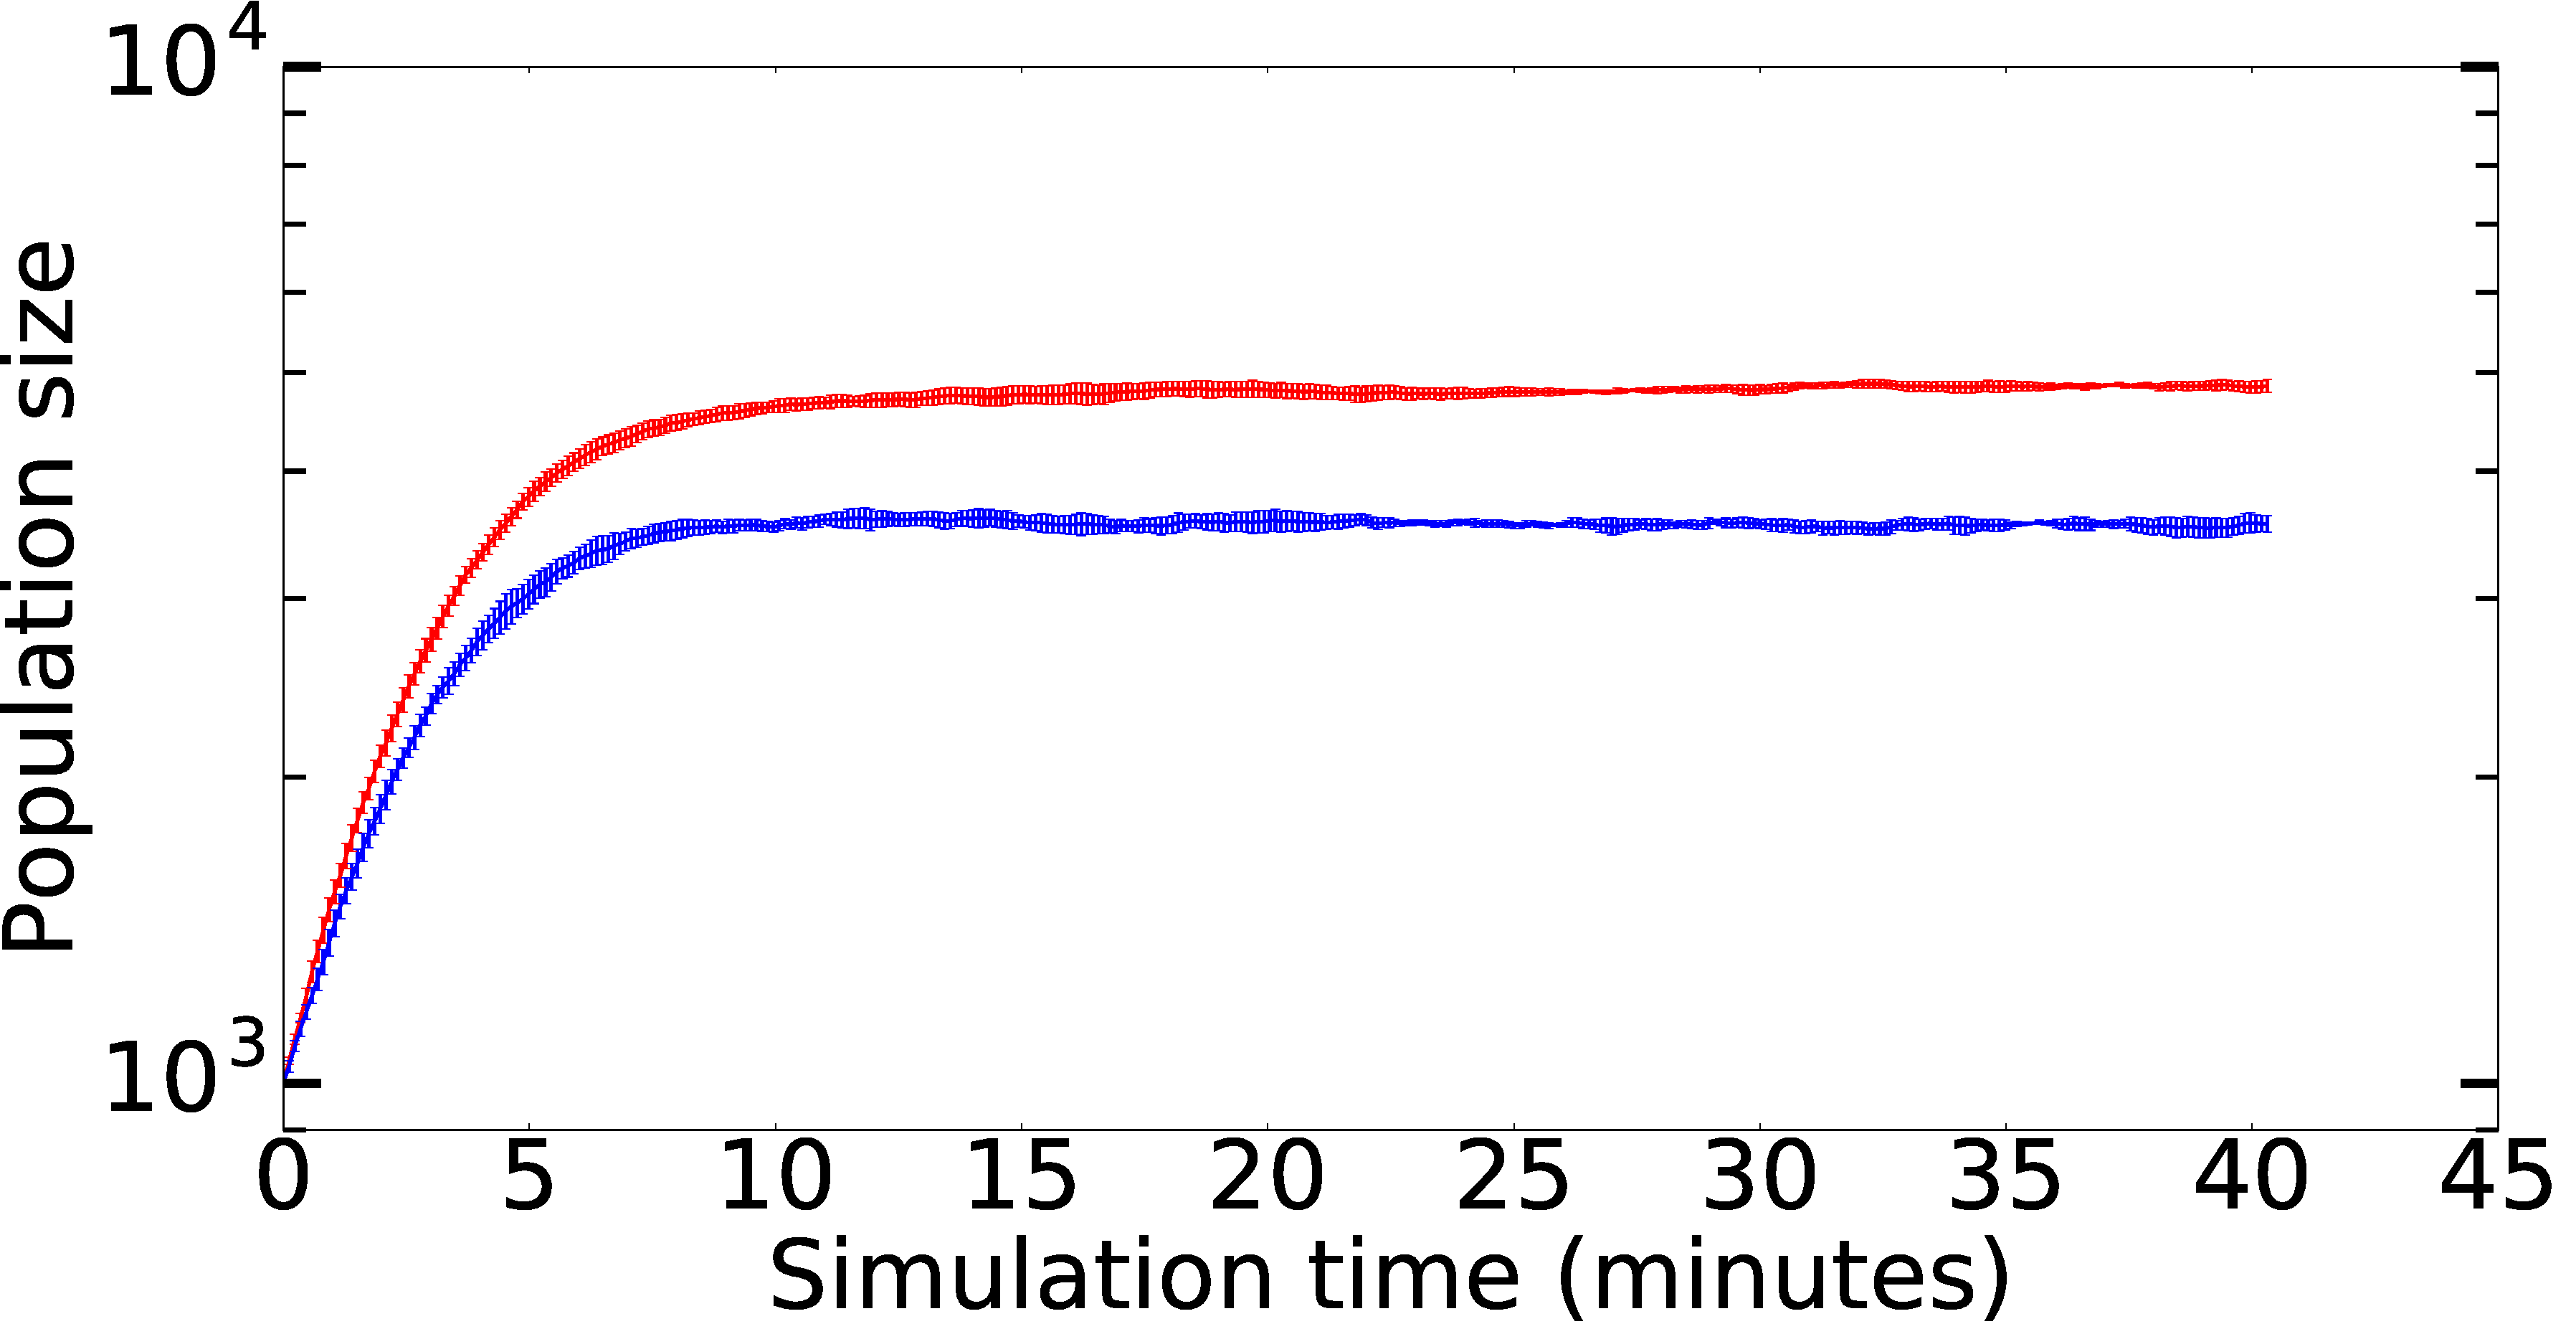
\includegraphics[width=0.9\columnwidth]{../dev/graphics/Jul18/const_pop.pdf}
      \end{center}


      \end{alertblock}
\end{column}
% ----------------------------------------------------------------
\begin{column}{\sepwid}\end{column} % Empty spacer column





\end{columns} % End of all the columns in the poster
\end{frame} % End of the enclosing frame

\end{document}
